\myChapter{Experiments}
\label{chap:Experiments}

% \section{TODOs}
% \begin{itemize}
% 
% \item{increase precision of times table}
% \item{decrease precision of metrics table and add VMAF}
% \item{make figure captions shorter and describe such images}
% \item{adjust figures positioning}
% \item{include table to showcase memory consumption differences}
% 
% \item{explain the following:
%   From \cref{tab:tab1}, INT8 models outperform full-precision performance on non-perceptual metrics, such as SSIM, PSNR, MS-SSIM. This is probably due to the fact that outputs from lower precision models are naturally more blurry than the ones from full-precision models.
% }
% 
% \item{explain the following:
%   Images generated by plain PyTorch implementations and their FP32 versions differ in quality most likely because they differ at the end of their architectures, since they use respectively bicubic and bilinear interpolation techniques to scale up the input low-quality image to allow the models to learn residual values between low- and high-quality images.
% }
% \end{itemize}


In this chapter, we will showcase various experiments and their corresponding results, highlighting the inference speed and image quality. We will utilize both the basic PyTorch implementations of UNet and SRUNet, as well as their compiled counterparts with TensorRT, which will be configured with different precisions for weights/activations, namely FP32, FP16, and INT8.

\section{Quantitative Results}
\label{sec:quantitative-results}

For each model variation, \cref{tab:metrics} reports the average value of each metric, along with its standard deviation. Higher values of these metrics indicate better image quality. The table shows that the UNet models have higher values for LPIPS and BRISQUE, but lower values for PSNR compared to the SRUNet models. However, the SSIM and MS-SSIM metrics are similar for both models. Additionally, there is a notable difference between the performance of the plain PyTorch implementations and their TensorRT counterparts for both UNet and SRUNet models, especially for LPIPS, BRISQUE, and PSNR metrics.

\begin{table*}[t]
\begin{tabular}{llllll}
\toprule
{} &          LPIPS &           SSIM &            PSNR &        MS-SSIM &         BRISQUE \\
\midrule
UNet        &  0.559 ± 0.007 &  0.879 ± 0.004 &  21.939 ± 0.027 &  0.735 ± 0.002 &   153.591 ± 0.0 \\
UNet\_FP32   &  0.354 ± 0.011 &  0.897 ± 0.003 &   28.64 ± 0.108 &  0.871 ± 0.003 &   26.783 ± 1.83 \\
UNet\_FP16   &  0.354 ± 0.011 &  0.897 ± 0.003 &   28.64 ± 0.108 &  0.871 ± 0.003 &   26.788 ± 1.84 \\
UNet\_INT8   &  0.343 ± 0.011 &  0.895 ± 0.003 &  28.613 ± 0.108 &   0.87 ± 0.003 &  26.448 ± 1.694 \\
SRUNet      &  0.551 ± 0.008 &  0.869 ± 0.004 &  19.303 ± 0.014 &  0.669 ± 0.002 &   153.591 ± 0.0 \\
SRUNet\_FP32 &  0.396 ± 0.012 &  0.896 ± 0.003 &  28.837 ± 0.126 &  0.871 ± 0.003 &  34.647 ± 2.336 \\
SRUNet\_FP16 &  0.396 ± 0.012 &  0.896 ± 0.003 &  28.837 ± 0.126 &  0.871 ± 0.003 &  34.642 ± 2.334 \\
SRUNet\_INT8 &  0.373 ± 0.012 &  0.895 ± 0.003 &  28.806 ± 0.124 &  0.869 ± 0.003 &  34.868 ± 1.989 \\
\bottomrule
\end{tabular}
\caption{Evaluation metrics over 50 frames (mean $\pm$ standard deviation).}
\label{tab:metrics}
\end{table*}

\begin{figure*}[ht]
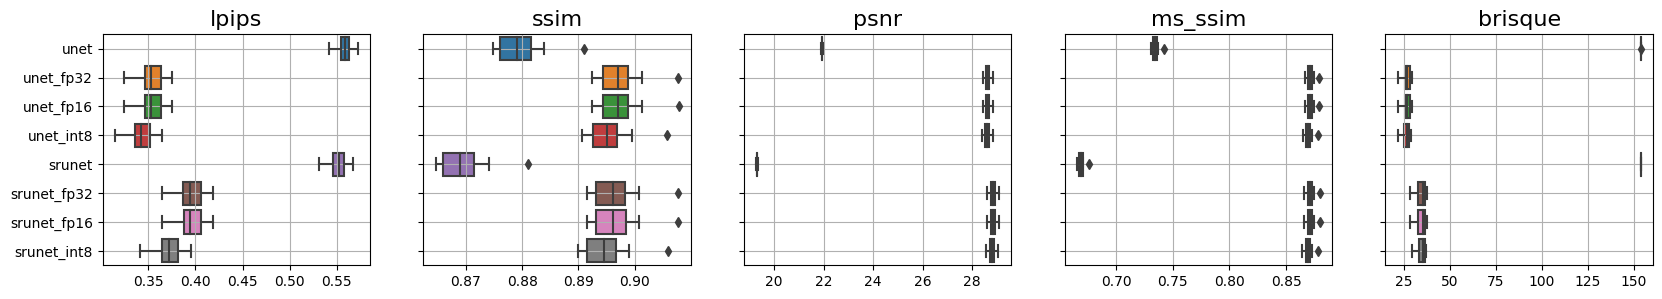
\includegraphics[width=1.0\textwidth]{static/2023_03_02_boxplots_metrics_all.png}
\caption{Box-plots for several metrics on validation images using different versions of UNet and SRUNet implementations.}
\label{fig:metrics}
\end{figure*}

\Cref{tab:timings} shows the execution times (in seconds) of different variations of UNet and SRUNet implementations. Each table entry represents the average execution time over more than 300 executions "$\pm$" its standard deviation. SRUNet generally has faster execution times than UNet across all versions. Among the different numerical precisions, the fastest execution times are generally achieved, as expected by using INT8, followed by FP16 and FP32.

The distributions of the execution times are shown in \cref{fig:timings-all}, zooming in for the compiled versions of the plain UNet (FP32/FP16/INT8) in \cref{fig:timings-unet}, as well as in \cref{fig:timings-srunet} for SRUNet.

\begin{table*}[t]
\begin{tabular}{ll}
\toprule
{} &      times [s] \\
\midrule
UNet        &    0.035 ± 0.0 \\
UNet\_FP32   &  0.028 ± 0.001 \\
UNet\_FP16   &  0.028 ± 0.001 \\
UNet\_INT8   &    0.015 ± 0.0 \\
SRUNet      &    0.012 ± 0.0 \\
SRUNet\_FP32 &  0.009 ± 0.001 \\
SRUNet\_FP16 &    0.009 ± 0.0 \\
SRUNet\_INT8 &    0.006 ± 0.0 \\
\bottomrule
\end{tabular}
\caption{Evaluation times over 1000 runs (mean $\pm$ standard deviation).}
\label{tab:timings}
\end{table*}

% \begin{figure*}[ht]
% 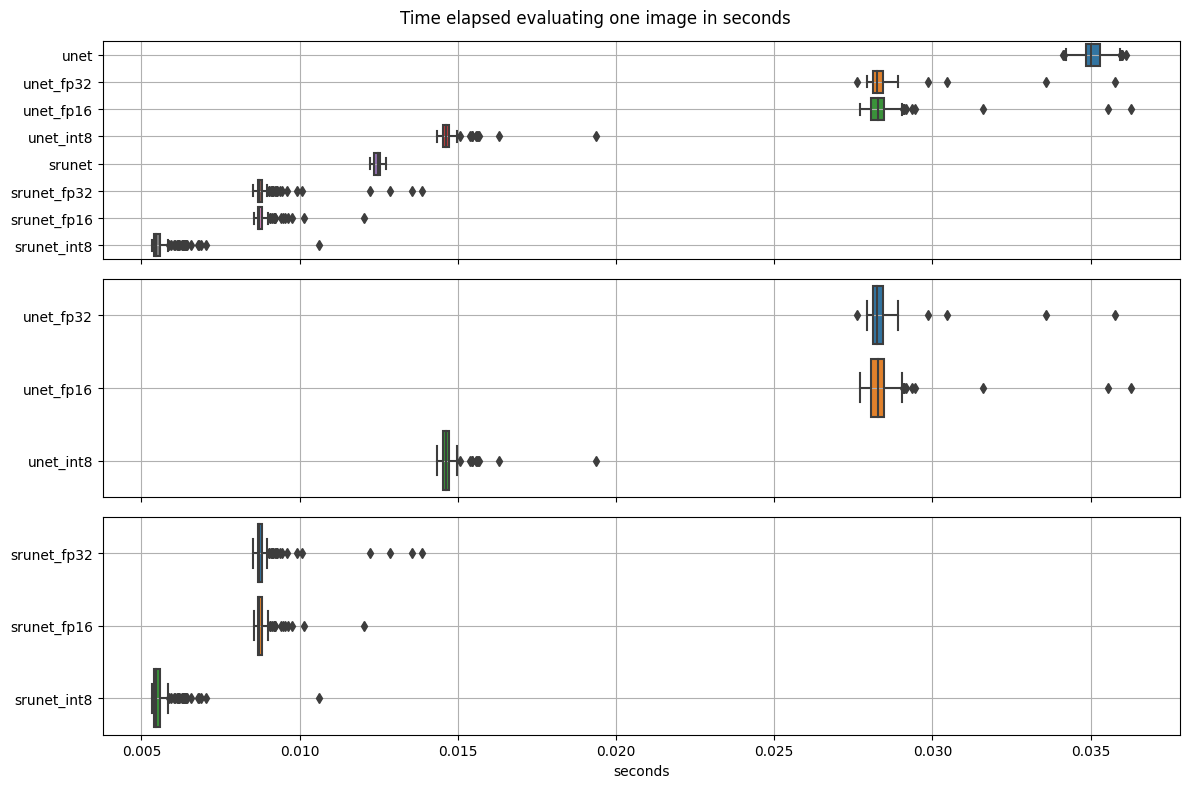
\includegraphics[width=1.0\textwidth]{static/2023_03_02_boxplots_timings_all.png}
% \caption{Average times elapsed in seconds for generating one image using different versions of UNet and SRUNet implementations. The top graph shows all the versions, and the middle one zooms in comparing only the 
% TensorRT versions of UNet, as well as the bottom graph for SRUNet.}
% \label{fig:timings-all}
% \end{figure*}
% 
% \begin{figure*}[ht]
% \includegraphics[width=1.0\textwidth]{static/2023_03_02_boxplots_metrics_quant_UNet.png}
% \caption{Box-plots for several metrics on validation images using UNet compiled in TensorRT (FP32/FP16/INT8).}
% \label{fig:timings-unet}
% \end{figure*}
% 
% \begin{figure*}[ht]
% \includegraphics[width=1.0\textwidth]{static/2023_03_02_boxplots_metrics_quant_SRUNet.png}
% \caption{Box-plots for several metrics on validation images using SRUNet compiled in TensorRT (FP32/FP16/INT8).}
% \label{fig:timings-srunet}
% \end{figure*}
% 
% \begin{figure*}[ht]
% 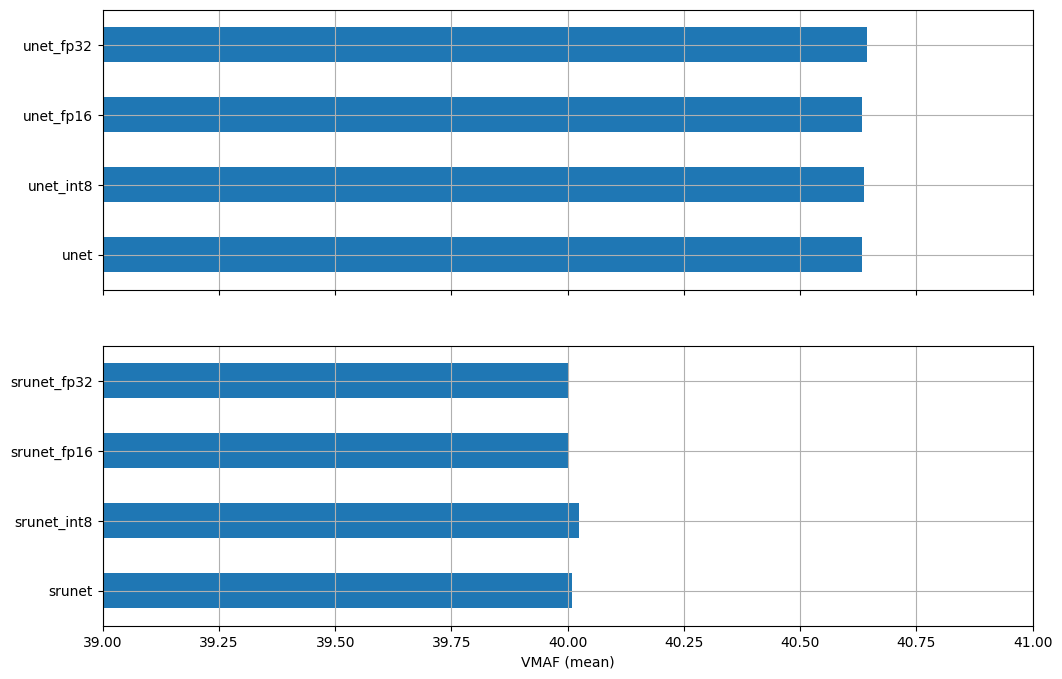
\includegraphics[width=1.0\textwidth]{static/2023_03_17_barplot_vmaf_mean.png}
% \caption{Mean VMAF score on a test video using different versions of UNet and SRUNet implementations.}
% \label{fig:vmaf-mean}
% \end{figure*}
% 
% \begin{figure*}[ht]
% 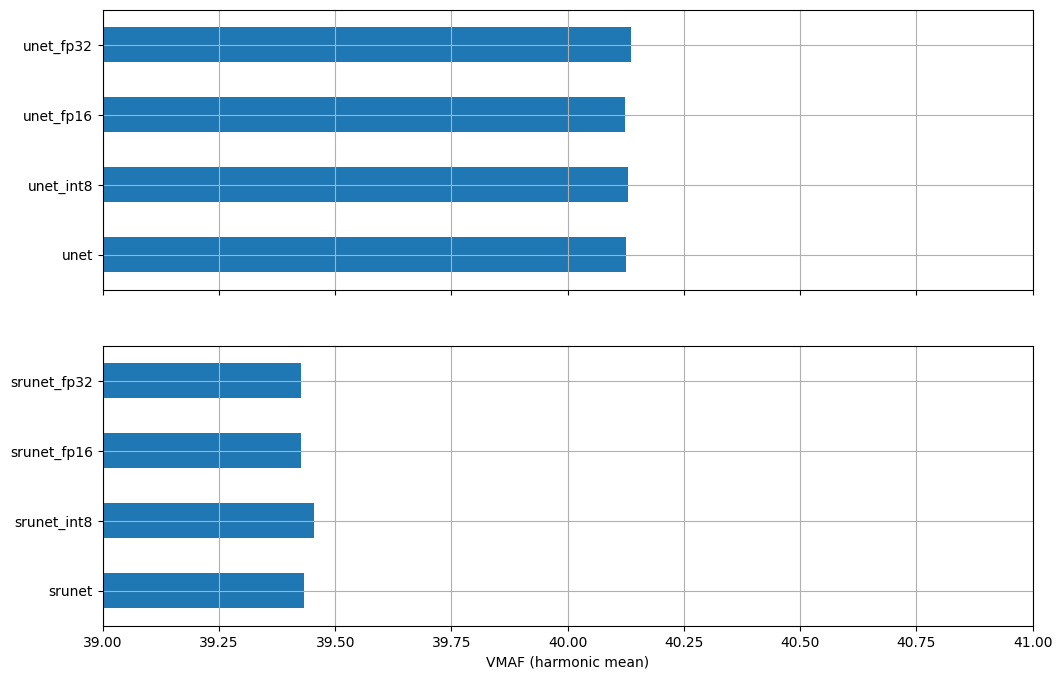
\includegraphics[width=1.0\textwidth]{static/2023_03_17_barplot_vmaf_harmonic_mean.png}
% \caption{Harmonic mean VMAF score on a test video using different versions of UNet and SRUNet implementations.}
% \label{fig:vmaf-harmonic-mean}
% \end{figure*}
% 
% \clearpage
% 
% \section{Qualitative Results}
% \label{sec:qualitative-results}
% 
% \begin{figure*}[ht]
% \includegraphics[width=1.0\textwidth]{static/2023_03_24_qualitative_unet.jpg}
% \caption{UNet qualitative results: (left) high-quality image; (center) generated image; (right) low-quality image.}
% \label{fig:qualitative-unet}
% \end{figure*}
% 
% \begin{figure*}[ht]
% \includegraphics[width=1.0\textwidth]{static/2023_03_24_qualitative_unet_fp32.jpg}
% \caption{UNet FP32 qualitative results: (left) high-quality image; (center) generated image; (right) low-quality image.}
% \label{fig:qualitative-unet-fp32}
% \end{figure*}
% 
% \begin{figure*}[ht]
% \includegraphics[width=1.0\textwidth]{static/2023_03_24_qualitative_unet_fp16.jpg}
% \caption{UNet FP16 qualitative results: (left) high-quality image; (center) generated image; (right) low-quality image.}
% \label{fig:qualitative-unet-fp16}
% \end{figure*}
% 
% \begin{figure*}[ht]
% \includegraphics[width=1.0\textwidth]{static/2023_03_24_qualitative_unet_int8.jpg}
% \caption{UNet INT8 qualitative results: (left) high-quality image; (center) generated image; (right) low-quality image.}
% \label{fig:qualitative-unet-int8}
% \end{figure*}
% 
% \begin{figure*}[ht]
% \includegraphics[width=1.0\textwidth]{static/2023_03_24_qualitative_srunet.jpg}
% \caption{SRUNet qualitative results: (left) high-quality image; (center) generated image; (right) low-quality image.}
% \label{fig:qualitative-srunet}
% \end{figure*}
% 
% \begin{figure*}[ht]
% \includegraphics[width=1.0\textwidth]{static/2023_03_24_qualitative_srunet_fp32.jpg}
% \caption{SRUNet FP32 qualitative results: (left) high-quality image; (center) generated image; (right) low-quality image.}
% \label{fig:qualitative-srunet-fp32}
% \end{figure*}
% 
% \begin{figure*}[ht]
% \includegraphics[width=1.0\textwidth]{static/2023_03_24_qualitative_srunet_fp16.jpg}
% \caption{SRUNet FP16 qualitative results: (left) high-quality image; (center) generated image; (right) low-quality image.}
% \label{fig:qualitative-srunet-fp16}
% \end{figure*}
% 
% \begin{figure*}[ht]
% \includegraphics[width=1.0\textwidth]{static/2023_03_24_qualitative_srunet_int8.jpg}
% \caption{SRUNet INT8 qualitative results: (left) high-quality image; (center) generated image; (right) low-quality image.}
% \label{fig:qualitative-srunet-int8}
% \end{figure*}
% 
